\section{Fragen zu Vorlesung 4}

\subsection{Welches Frequenzspektrum hat ein sinusförmiges, welchess ein Pulsförmiges Signal?}
Siehe Fragen~\ref{sec:lv3:freq_spekt}
\begin{itemize}
  \item \textbf{Sinus:} Einzelner Puls bei der Frequenz des Signals
  \item \textbf{Puls:} Hoher Puls bei der Frequenz des Signals. Langsam absinkende Pulse bei Vielfachen der Grundfrequenz. (Höherer Puls bei ungeraden Vielfachen)
\end{itemize}

\subsection{Wann und warum entstehen elektrostatische Aufladungen?}\label{sec:lv4:electrostatic}
Durch große Potentialdifferenzen entstehende Spannungsdurchschläge (durchdringen eines Isolators). Diese Durchschläge bewirken einen kurzen, hohen elektrischen Strom\p
z.B.
\begin{itemize}
  \item Reiben von isolierenden Stoffen
  \item Pos. Ladungsüberschuss auf Glasstab bei Reiben mit Wolle
  \item Auf Textilboden gehende Person -> Aufladung der Person
\end{itemize}

\subsection{Mit welchen Spannungs- und Stromhöhen ist bei ESD zu rechnen?}
\begin{itemize}
  \item Amplituden bis 30kV
  \item Entladeströme 10 bis 100A
\end{itemize}

\subsection{Welche Parameter haben Einfluss auf elektrostatische Aufladungen?}


\subsection{Welches Frequenzspektrum hat ein ESD Puls?}
Breitbandiges Störspektrum

%TODO Foto ESD Entladung Prüfimpuls EN 61000-4-2

\subsection{Welche Anstiegszeit und welche Halbwertszeit hat ein ESD Puls?}
Sehr schnelle Anstiegszeiten Subnanobereich
~ 30 ns Halbwertszeit

\subsection{Wie kann ein ESD Puls in elektronische Schaltungen einkoppeln?}
\begin{itemize}
  \item Galvanisch durch Funkenüberschlag
  \item Induktiv durch di/dt auf geerdete Teile
  \item Kapazitiv durch du/dt auf isolierte metallische Teile
  \item Abstrahlung Magnetfeld durch große di/dt
\end{itemize}

\subsection{Was versteht man unter einen triboelektrischen Effekt?}
Engl.: Triboelectric Charge. Elektrostatische Aufladung durch Berührung/Reibung (Siehe Frage~\ref{sec:lv4:electrostatic}). Verschiebung von Elektronen auf der Metalloberfläche meist durch Berührung und anschließender Trennung. => Ladungstransfer zwischen Körpern mit verschiedenem Potential.

\subsection{Welche Maßnahmen werden zum Schutz von elektrostatischer Entladung gesetzt?}
Abhilfe: ESD-Schutzelemente
\begin{itemize}
  \item ESD Schutzbeschaltung TVS-Dioden
\end{itemize}

\subsection{Was ist der Unterschied zwischen dem HBM und dem MM?}

\subsection{Was ist der Unterschied zwischen Kontakt und Luftentladung? Wann wird welche Entladeart angewandt?}
\textbf{Kontaktentladung}
%TODO Definition
%
\begin{itemize}
  \item gezielt
  \item reproduzierbar
  \item direkt/indirekt
\end{itemize}
%
\textbf{Luftentladung}
%TODO Definition
%
\begin{itemize}
  \item ungezielt
  \item schlecht reproduzierbar
\end{itemize}

\subsection{Von welchen Einflüssen ist die Reproduzierbarkeit der ESD Luftentladung abhängig?}
\begin{itemize}
  \item Ladespannung
  \item Annäherungsgeschwindigkeit
  \item Umgebungsdruck
  \item Luftfeuchtigkeit
\end{itemize}

\subsection{Wie schaut ein ESD Prüfaufbau aus?}
%TODO Foto ESD Entladung Prüfaufbau (direkt)

\subsection{Wann und warum entstehen Burststörungen?}
Burststörungen sind leitungsgeführte Störungen und treten bei schnellen Schaltflanken auf. 

\subsection{Welches Frequenzspektrum hat ein Burstpuls?}

\begin{figure}[ht]
  \centering
  \includegraphics[height=7cm]{src/assets/pictures/VL_3_elektromagnetische_störungen.jpg}
  \caption{Elektromagnetische Störungen, Auftreten und Frequenzspektrum}
\end{figure}

\subsection{Mit welchen Spannungs- und Stromhöhen ist beim Burststörungen zu rechnen?}

\subsection{Welche Anstiegszeit und welche Halbwertszeit hat ein Burstpuls?}

\subsection{Wie viele Pulse hat ein Burstpaket?}

\subsection{Welche Einkopplungsmöglichkeiten kennt man bei der Burstprüfung?}

\subsection{Wie können Burststörungen in elektronischen Schaltungen reduziert werden?}

\subsection{Wann und warum entstehen Surgestörungen?}
Surgestörungen sind leitungsgeführte Störungen und treten bei Überspannungen durch einen Blitzeinschläge auf. 

\subsection{Welches Frequenzspektrum hat ein Surgepuls?}

\begin{figure}[ht]
  \centering
  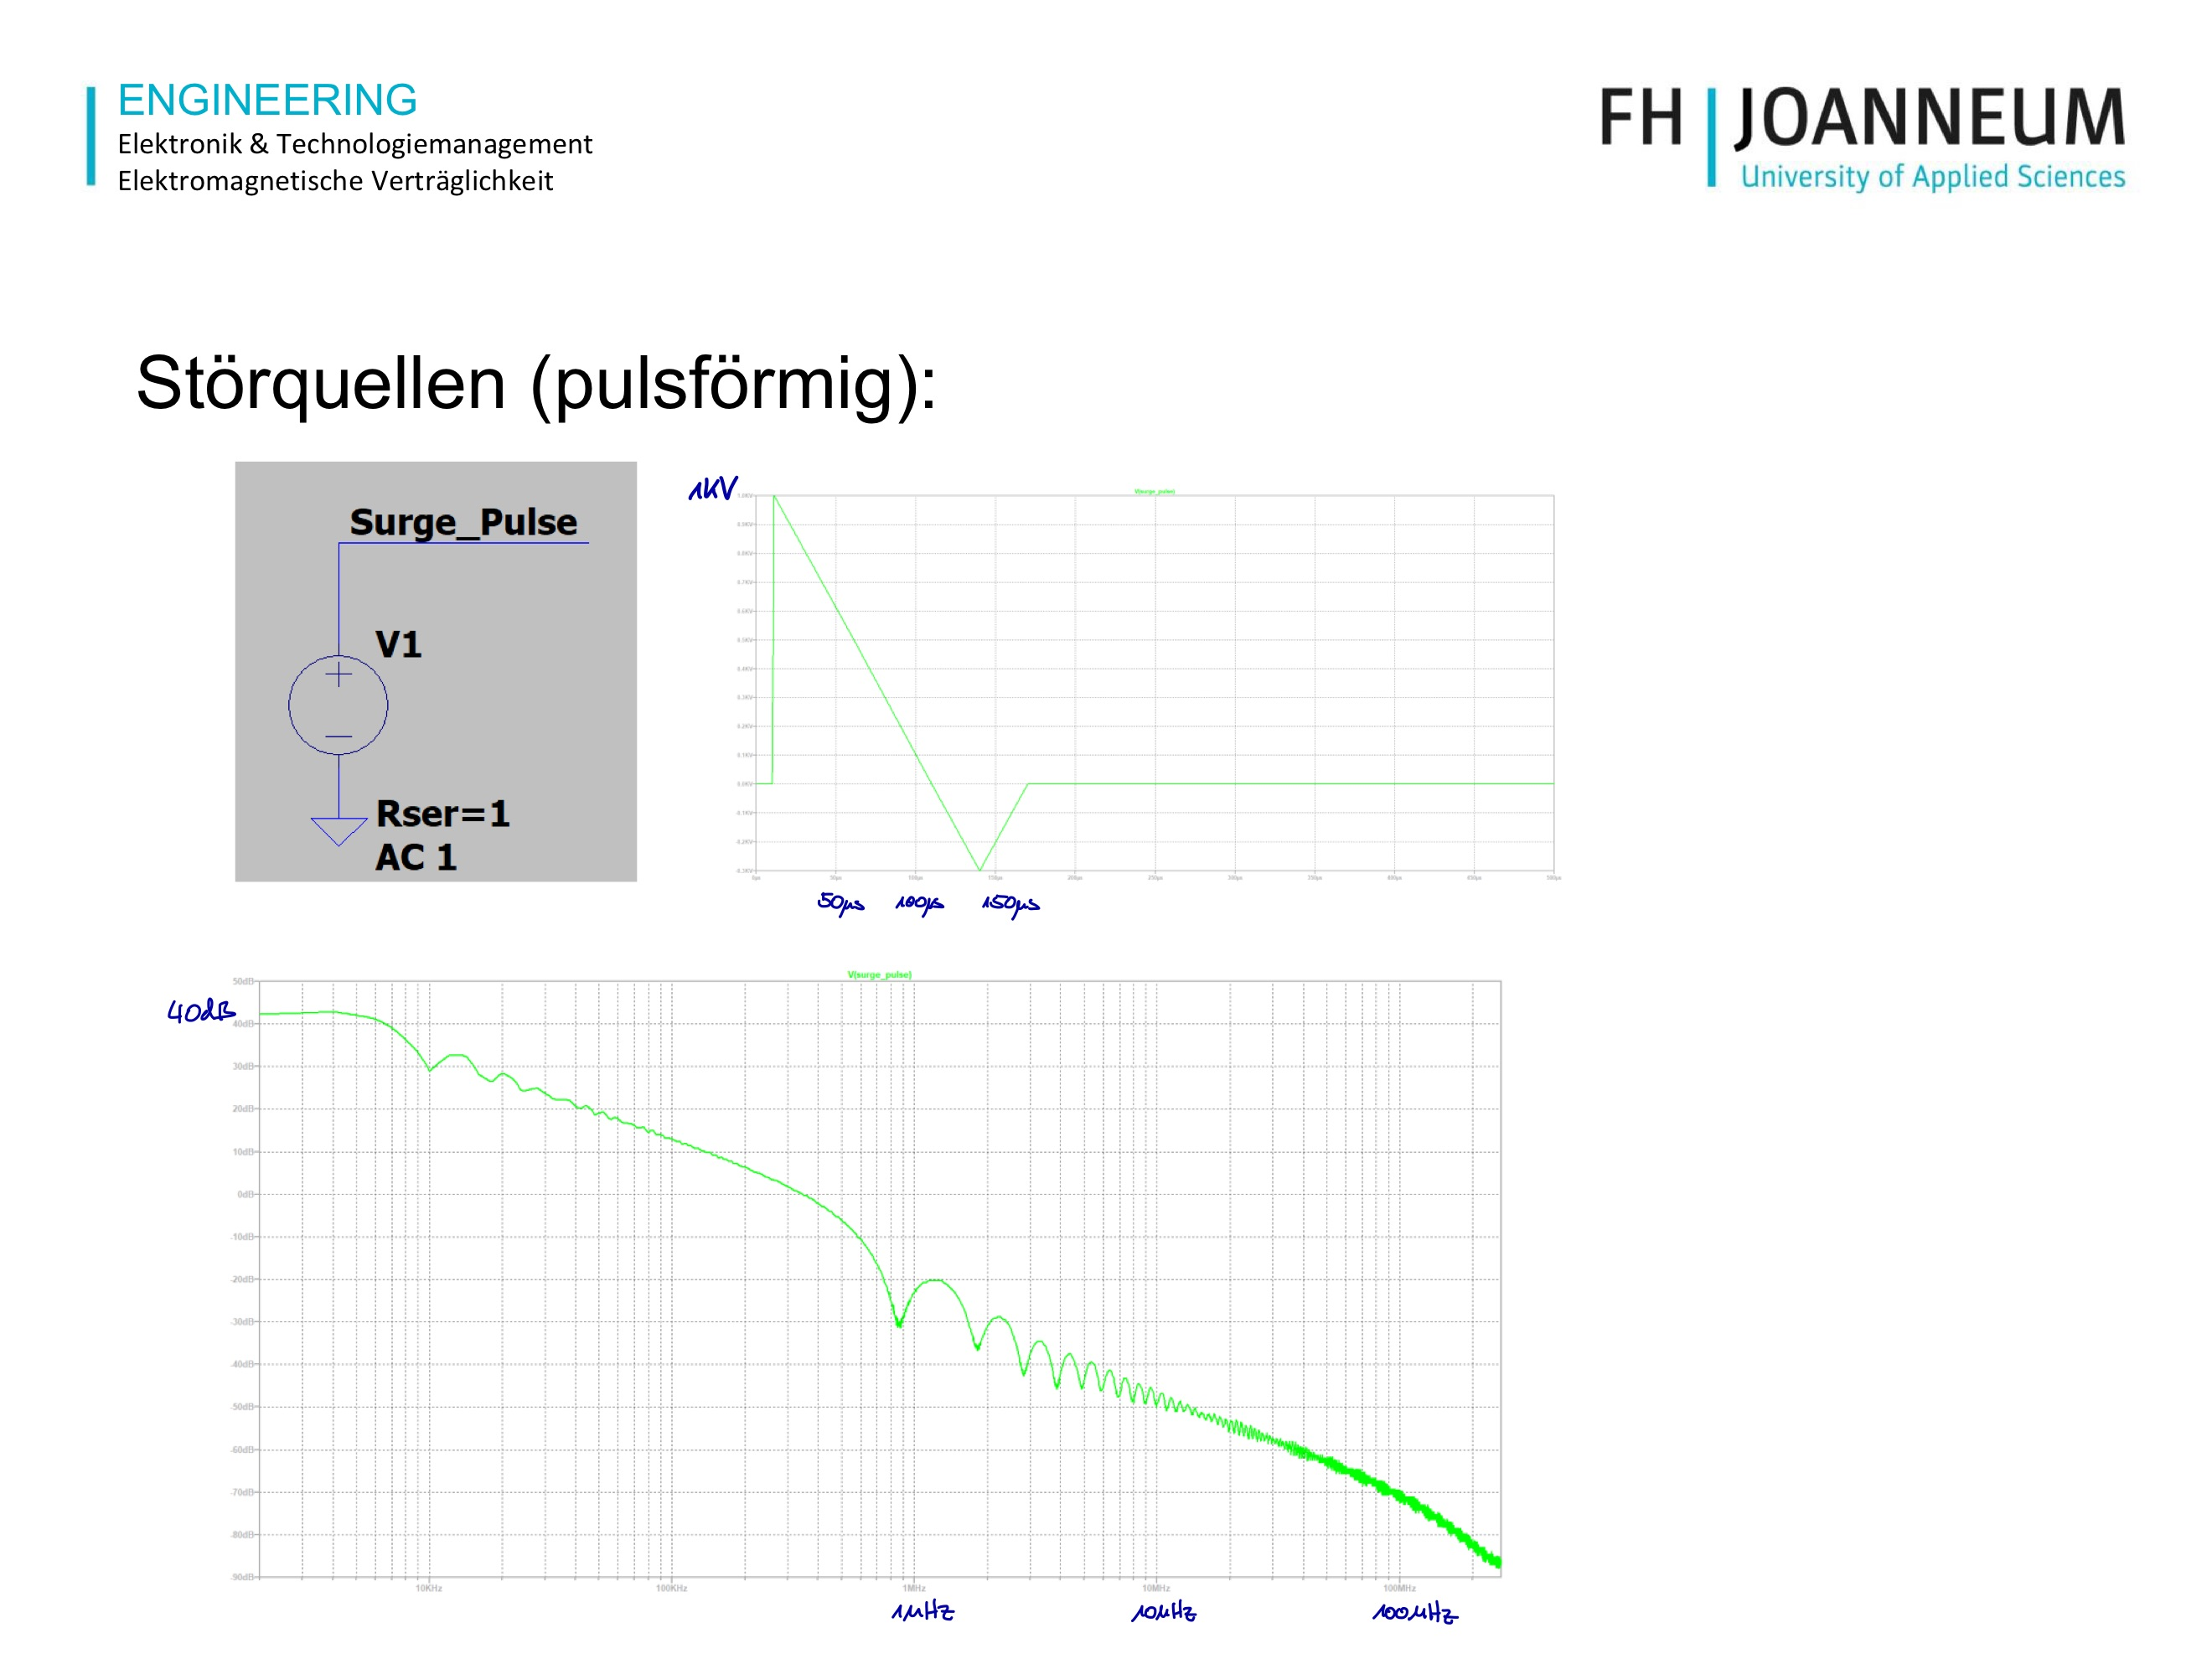
\includegraphics[height=7cm]{src/assets/pictures/VL_3_surge_pulse.jpg}
  \caption{Elektromagnetische Störungen, Auftreten und Frequenzspektrum}
\end{figure}

\subsection{Mit welchen Spannungs- und Stromhöhen ist beim Surge zu rechnen?}
Spannungen bis in den KV-Bereich

\subsection{Wie können elektronische Schaltungen vor Surge geschützt werden?}

\subsection{Auf welchen Leitungen werden Surge- und Burststörungen üblicherweise eingekoppelt?}

\pagebreak
